\documentclass{article}
\usepackage[utf8]{inputenc}

\title{Text Independent Speaker Authentication in Noisy Environments \\
        \large MLND Capstone Project}

\author{Abdullah AlOthman}
\date{March 2018}

\usepackage{natbib}
\usepackage{listings}
\usepackage{graphicx}
\usepackage{float}
\begin{document}

\maketitle
\section{Definition}

\subsection{Project Overview}

Speaker Authentication (or Verification) is the process of verifying the identity of a speaker based on the characteristics of their voice. This problem falls in the biometrics domain and there has been previous attempts to solve it using supervised learning \cite{Campbell2006SupportVM}, unsupervised learning \cite{Reynolds2000SpeakerVU} and of course using deep learning \cite{Nagrani17}. 

In this project, I'll attempt to solve this problem using a deep neural network model.


\subsection{Problem Statement} \label{prblmstmt}
Most implementations of speaker verification systems are dependant on specific phrases (e.g. " Hey, Google..", "Hey, Siri..", "Alexa..") and consistent audio-environment (same microphone, audio quality, etc).
What I want to tackle in this project is text-independent speaker verification, in noisy, uncontrolled environments.

Applications of speaker verification include:
\begin{itemize}
    \item authentication in high-security systems
    \item authentication in forensic tests
    \item searching for persons in large corpora of speech data
\end{itemize}
All of these applications require reliable performance in ‘wild’ conditions (i.e. real-world scenarios). The challenges expected in this task come from two main fronts:
\begin{enumerate}
    \item High variance in the environment (background music, crowds, recording quality, etc.)
    \item High variance in the speaker age, accent, emotion, intonation, etc.
\end{enumerate}

I will attempt to solve this problem by building a neural network model that will take as input the features we've extracted from two speaker-audios and outputs the probability of a speaker match.
\subsection{Metrics}
To evaluate the model, I'm choosing Equal Error Rate $(EER)$ as the performance metric.
For each authentication pair the model outputs a continuous variable $X$, which is the estimated probability of a match.

Given a threshold parameter $T$, the instance is accepted as a match if $X>T$, and rejected otherwise.
$X$ follows a probability density $f_1(x)$
if the instance is actually a match, and $f_0(x)$ otherwise \cite{wiki:xxx}.

The false rejection rate is given by 
\begin{equation}
FRR(T) = 1- \int_{T}^\infty f_1(x) \, dx
\end{equation}
and the false acceptance rate is given by 
\begin{equation}
\mbox{FAR}(T)= \int_{T}^\infty f_0(x) \, dx 
\end{equation}. 

EER is defined as the rate at the threshold $T$ where $FRR(T) = FAR(T)$ (see Figure \ref{fig:EER}).
EER is commonly used as a performance metric for  identity-verification systems, as it balances the rate at which false-acceptance and false-rejection occurs. The lower the EER value, the higher the accuracy of the system. EER is also the metric used by for our benchmark model.

\begin{figure}[H]
    \centering
    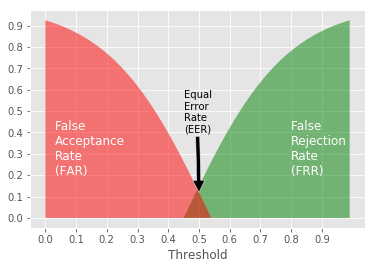
\includegraphics[scale=.75]{images/eer.png}
    \caption{EER Visualized in an Example}
    \label{fig:EER}
\end{figure}

\section{Analysis}

\subsection{Data Exploration and Visualization}

for this problem, I'm using the VoxCeleb dataset\cite{Nagrani17}.
VoxCeleb dataset was created by extracting audio from YouTube videos.
it contains over 100,000 utterances for 1251 celebrities. The speakers are gender balanced and span a wide range of different ethnicities, accents, and ages.


This dataset includes varying audio qualities and challenging acoustic environments, such as:
\begin{itemize}
    \item red carpet interviews
    \item outdoor stadium
    \item studio interviews
    \item speeches with large audience
    \item high production multimedia
    \item amateur multimedia (e.g. Vlogs)
\end{itemize}

The dataset also includes uncontrolled, real-world noise such as background-chatter, audience reactions, room acoustics, etc.
Table \ref{tab:stats_1} gives some idea of the distribution contained in the dataset.

In Figure \ref{fig:stats_2}, you'll see the nationality distribution of the speakers in this dataset. Which gives incite into the distribution of ethnicitis and accents. 


\begin{table}[H]
    \centering
    \begin{tabular}{ |c||c|c|c|  }
    \hline
    \multicolumn{2}{|c|}{number of speakers} & \multicolumn{2}{|c|}{1251} \\
    \hline
    \multicolumn{2}{|c|}{number of male speakers} & \multicolumn{2}{|c|}{690} \\
    \hline
     & max & average & min \\
     \hline
    videos per speaker & 36 & 18 & 8 \\
    \hline
    utterances per speaker & 250 & 116 & 45 \\
    \hline
    length of utterances (seconds) & 145.0 & 8.2 & 4.0 \\
    \hline
    \end{tabular}
    \caption{dataset statistics}
    \label{tab:stats_1}
\end{table}
\begin{figure}[H]
    \centering
    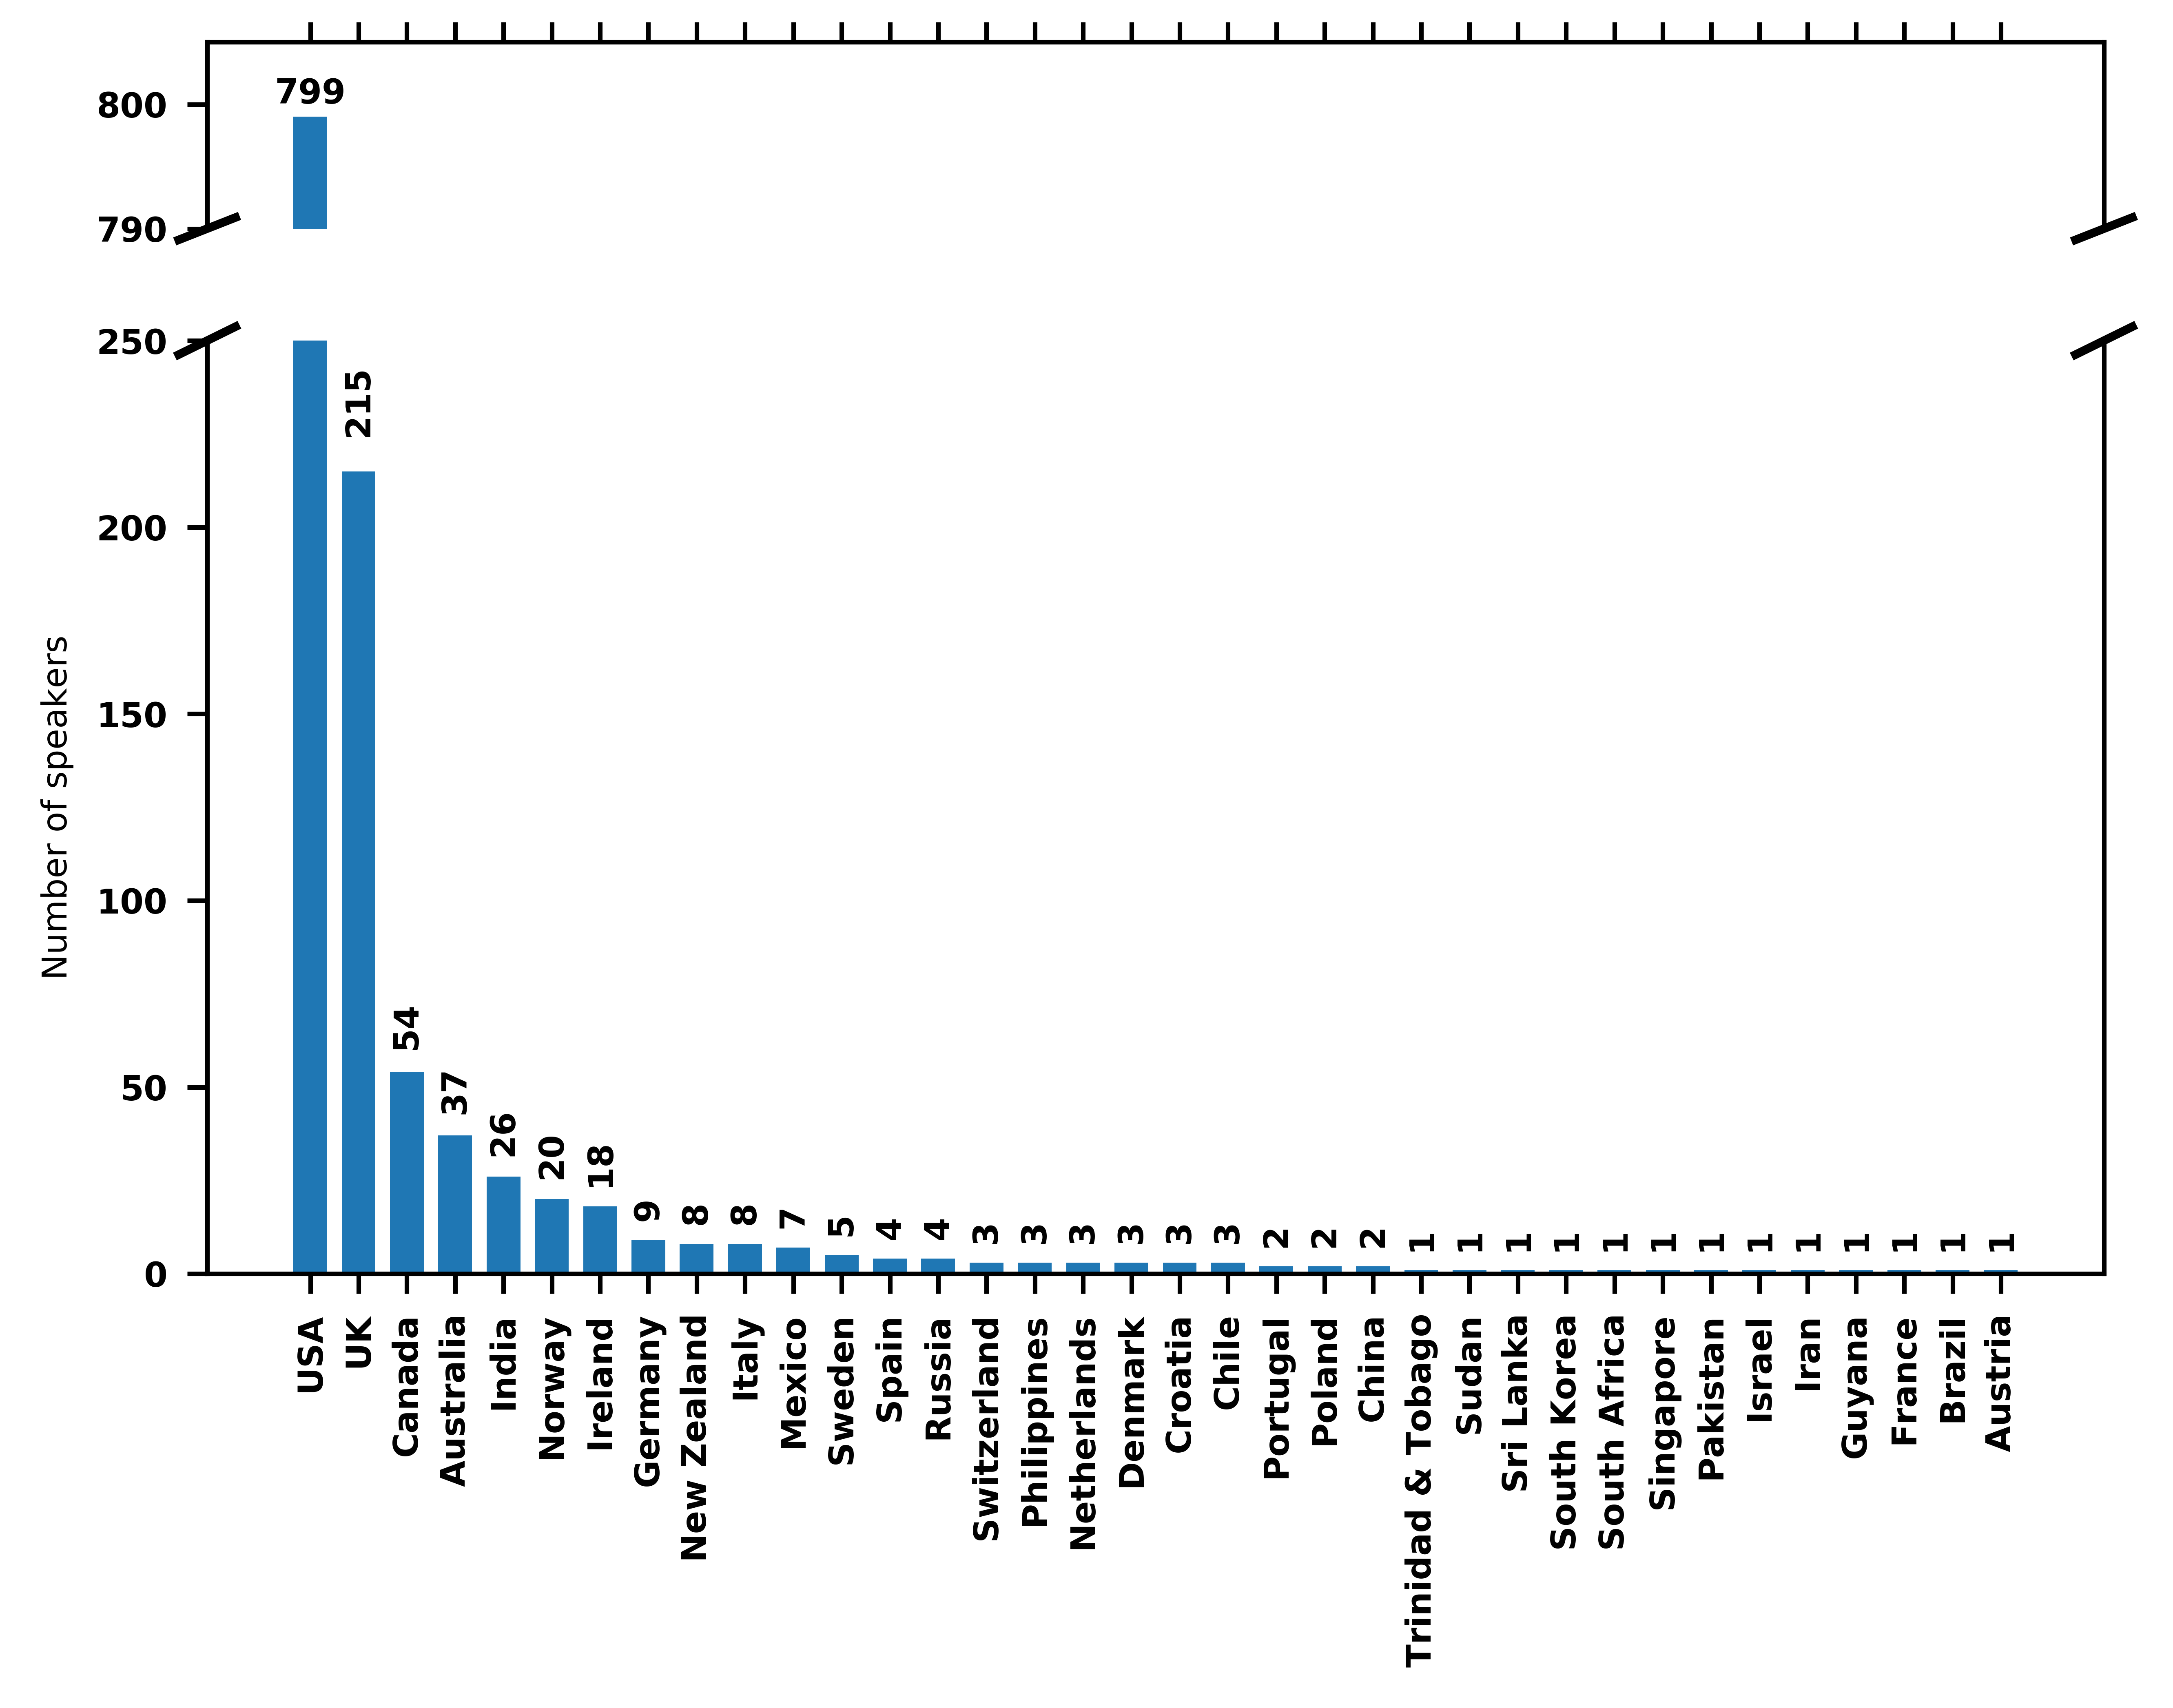
\includegraphics[scale=.75]{images/country.png}
    \caption{Nationality distribution}
    \label{fig:stats_2}
\end{figure}

\subsection{Algorithms and Techniques}
Since speech is inherently temporal, I decided to take that into account and chose a Recurrent Neural Network (RNN) as the basis of my model.

RNNs are a type of neural network that take into account the temporal relation between the input features (the value of $X_t$ affects the value of $X_{t+1}$). As an example from our data the audio features at the $t=0$ of an utterance informs the model on how to handle the features at $t=1$.

The big drawback that one might face when using neural networks in general is not having enough data, which fortunately is not an issue in this case since our dataset is large.

To be able to verify, you must first be able to identify. The first step I will do is train an identification model that takes as input features extracted from a given audio file and outputs the probability of who it thinks the speaker is.

Once the identification model is trained, I'll use it as a base for the verification model, which will take audio features extracted from 2 audio files as input and outputs the probability of a speaker match.

\subsection{Benchmark}

I'll be comparing my model to multiple benchmarks.

\begin{enumerate}
    \item Random Classifier: the most basic benchmark, but important to know we're preforming better than random chance.
    \begin{itemize}
        \item EER = 0.50
    \end{itemize}
    \item The GMM-UBM model proposed in the VoxCeleb paper.
    \begin{itemize}
        \item EER = 0.15
    \end{itemize}    
    \item The Embedding model proposed in the VoxCeleb paper.
    \begin{itemize}
        \item EER = 0.08
    \end{itemize}
\end{enumerate}

\section{Methodology}
\subsection{Data Preprocessing}
since the audio length is not consistent, I only considered the first 3 seconds of each utterance as inputs to the model. 

for feature extraction I used MFCC. Mel Frequency Cepstral Coefficents (MFCCs) are the state-of-the-art method for extracting audio features for speech and speaker recognition tasks. it is applied by first framing the signal into overlapping frames (standard parameters are 25ms length with 10ms overlap). Then applying log filterbank on periodogram estimate of the power spectrum. Then finally taking the Discrete Cosine Transform (DCT) coefficients of the log-filterbanks.\cite{jlyon}

Given the noisy state of the dataset, I then normalized with respect to the mean and the variance to get the CMVN features, Figure \ref{fig:normalizatin} shows how normalization boosts the signal to noise ratio.

\begin{figure}[H]
    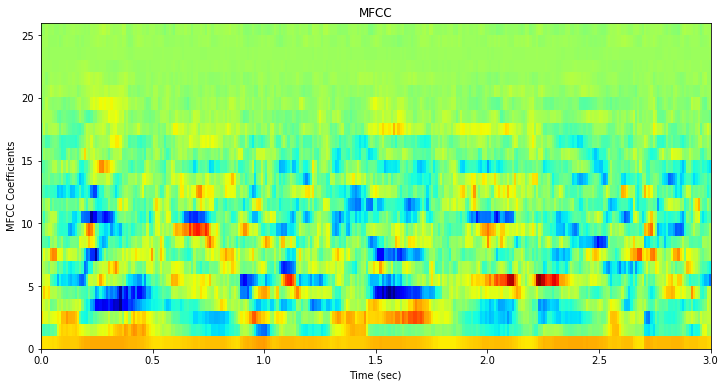
\includegraphics[scale=.5]{images/mfcc.png}
    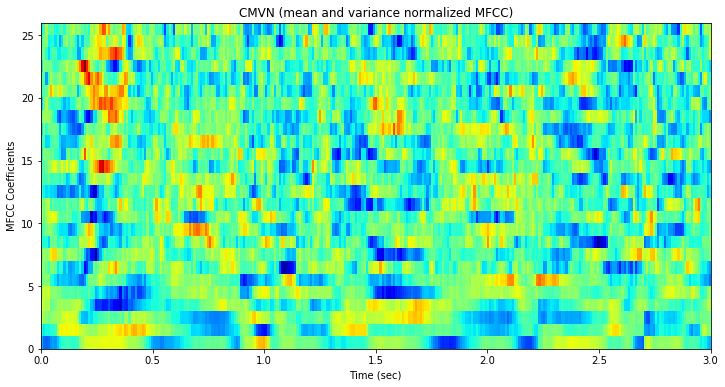
\includegraphics[scale=.5]{images/cmvn.png}
    \caption{MFCC before and after normalization}
    \label{fig:normalizatin}
\end{figure}

\subsection{Implementation} \label{implementation}
I first attempted to tackle the verification task directly using a convolutional neural network. That effort proved fruitless as I got results that were worse than random. I then started working on an identification model, using the same train/val/test split used in assessing the base model. I attempted to use different features such as the signal's spectogram and the log-filterbank but they were computationally expensive to extract and store, which is how I finally settled on using MFCCs.

I had no luck with CNNs even in the identification task. So I used the same architecture that I've been using in Kaggle's Toxic Comment Classification Challenge even though they operate on different data types (text/audio).

And to my delight, the model actually preformed well! (see table \ref{tab:id_results}).

The identification model's architecture is as follows:
\begin{itemize}
    \item input layer 
    \item Spatial Dropout layer: prevents the neural network from over-fitting by deactivating feature maps with a given probability
    \item bidirectional RNN: takes into account the temporal relation between the input features ( the value of $X_t$ affects the value of $X_{t+1}$)
    \item concatenated global max pooling and global average pooling
    \item Dropout:  prevents the neural network from over-fitting by deactivating neurons with a given probability
    \item Batch Normalization: forces the activations of the previous layer to have a gaussian distribution.
    \item output layer with Softmax activation
\end{itemize}
See figure \ref{fig:id_arch} for the architecture and table \ref{tab:id_results} for the results of the identification model.
\begin{figure}[H]
    \centering
    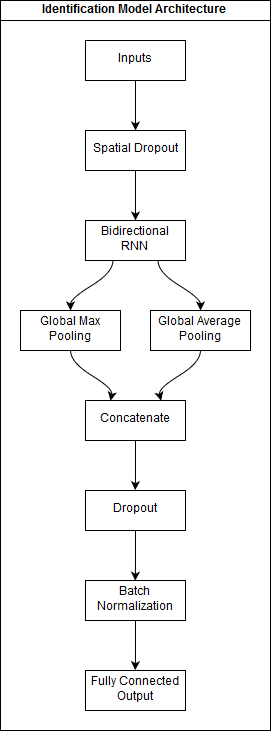
\includegraphics[scale=.65]{images/id_model.png}
    \label{fig:id_arch}
\end{figure}
\begin{table}[H]
    \centering
    \begin{tabular}{l*{6}{c}r}
        Model & Top - 1 & Top - 5\\
        \hline
        GRU - MFCC & 0.56 & 0.76  \\
        GRU - CMVN & 0.66 & 0.84  \\
        LSTM - CMVN & 0.68 & 0.85  \\
    \end{tabular}
    \caption{Top-1 and Top-5 Accuracy of the identification models}
    \label{tab:id_results}
\end{table}
For verification, I first created training pairs by creating balanced positive samples and negative samples for each utterance, where utterances must come from different video sources to be in a pair (for added difficulty). I then reserved a set of speakers for testing, these speakers are not included in the training set for either the verification or the identification models.
After that I froze the weights of the identification model and used them for my verification architecture (see figure \ref{fig:ver_arch}).
I used ReLU activation for the middle Dense layers and Sigmoid activation for the final layer

\begin{figure}[H]
    \centering
    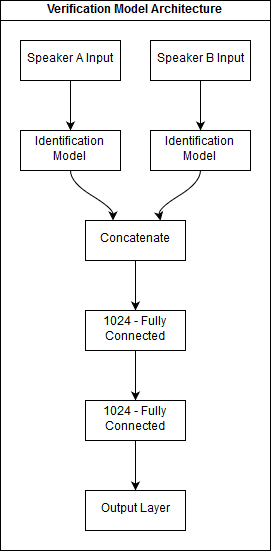
\includegraphics[scale=.65]{images/verification_model.png}
    \label{fig:ver_arch}
\end{figure}

\subsection{Refinement}
Moving from CNNs to RNNs gave the most dramatic improvement. Beyond that, table \ref{tab:id_results} shows the improvements of using CMVNs instead of MFCCs and the marginal improvement of using LSTM over GRU.

As for Hyperparameter tuning, using Adam as the optimizer helped the model converge faster. That, combined with using high dropout rate (0.5) and batch normalization helped the model achieve better results.

\subsection{Coding Challenges}
most of the coding challenges faced during this project were solved by framing the exact problem in mind, then diving deeply into Keras's\cite{chollet2015keras} or numpy's documentation.
\section{Results}
\subsection{Model Evaluation and Validation}
The final model results can be seen in table \ref{tab:ver_results}.

Since the test set contains no overlap in terms of videos or speakers with the training set, I would say that the model is generalizing well with new data and that these results can be trusted.
\begin{table}[H]
    \centering
    \begin{tabular}{l*{6}r}
        Model & EER\\
        \hline
        GRU-based siamese network & 0.15  \\
        LSTM-based siamese network & 0.14  \\
        using ensemble blend of both & 0.13  \\
    \end{tabular}
    \caption{results of the verification models}
    \label{tab:ver_results}
\end{table}

\subsection{Justification}

The final solution is described in full in section \ref{implementation}.

The final results (as seen in table \ref{tab:ver_results}), are better than 2 of the 3 benchmarks chosen for comparison. The model is robust enough for the uses proposed in section \ref{prblmstmt}.
given more data as input, using longer utterances for example will reduce the likelihood of miss-classification exponentially.
\section{Conclusion}
In this project, a recurrent neural network that determines whether two audio segments come from the same speaker has been developed.  As it currently stands the model can still be used in production as mentioned in the previous section. The model exceeded 2 of the 3 proposed benchmarks which means that while the model has preformed well, there's still room for improvement.
\subsection{Improvement}
due to time and computational resource constraints, I've not been able to experiment with some of the approaches I have initiallly considered.

Possible venues of improvement include:
\begin{itemize}
    \item Instead of building the training set randomly, consider using hard negative sampling for a more robust model.
    \item Use segments longer than 3 seconds, or use multiple overlapping segments from each utterance.
    \item Invistigate different possible feature representations. such as i-vector, d-vectors and full spectograms.
    \item Revisit CNNs, as I feel like I'm missing something here that will become clear with more research.
\end{itemize}
\subsection{Reflections}
I started this project with no prior knowledge in the world of Bio-metrics or audio processing. Working in this new domain strengthened my research skills in ways that will help me with my future projects. I grew more familiar with the libraries and tools available to me. working with hardware constraints forced me to get creative in writing my code to be more memory efficient.
\pagebreak
\bibliographystyle{plain}
\bibliography{references}
\end{document}
